\documentclass[tikz, border=10pt]{standalone}
\usepackage{tikz}
\usepackage{amsmath}
\usetikzlibrary{shapes, calc, backgrounds, arrows.meta}

\begin{document}
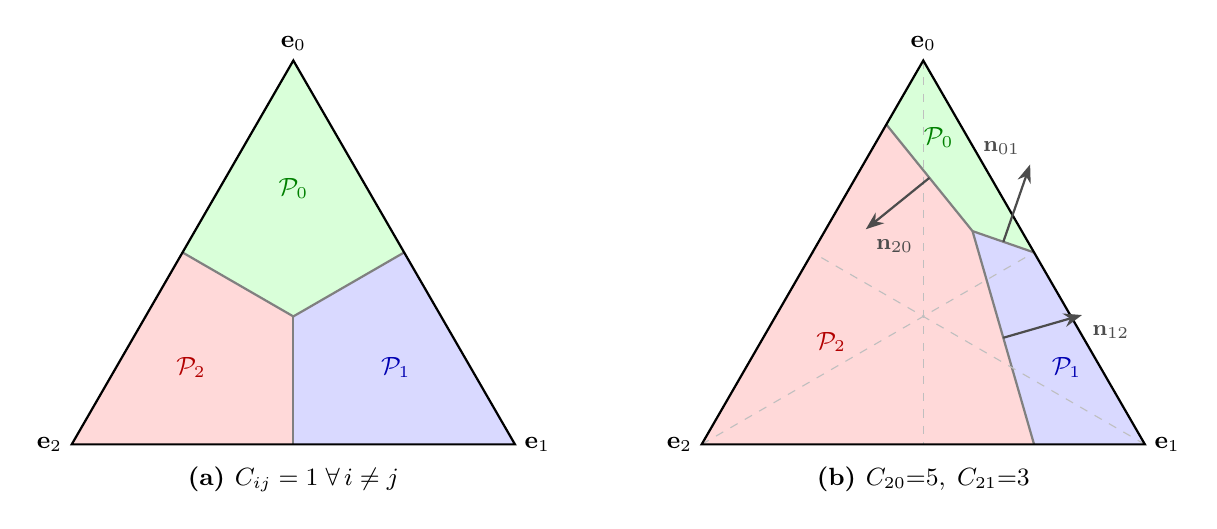
\begin{tikzpicture}[font=\sffamily]

    \begin{scope}[xshift=0.0cm, scale=0.65]
    \coordinate (Top) at (0.000, 5.000);
    \coordinate (Right) at (4.330, -2.500);
    \coordinate (Left) at (-4.330, -2.500);

    \coordinate (Int) at (0.000, 0.000);

    \fill[green!15] (0.000, 5.000) -- (2.165, 1.250) -- (0.000, 0.000) -- (-2.165, 1.250) -- cycle;
    \fill[blue!15] (4.330, -2.500) -- (0.000, -2.500) -- (0.000, 0.000) -- (2.165, 1.250) -- cycle;
    \fill[red!15] (-4.330, -2.500) -- (-2.165, 1.250) -- (0.000, 0.000) -- (0.000, -2.500) -- cycle;

    \draw[thick, black!50] (Int) -- (2.165, 1.250);
    \draw[thick, black!50] (Int) -- (-2.165, 1.250);
    \draw[thick, black!50] (Int) -- (0.000, -2.500);

    \draw[thick] (Top) -- (Right) -- (Left) -- cycle;

    \node[green!50!black, font=\small\bfseries] at (0.000, 2.500) {$\mathcal{P}_0$};
    \node[blue!70!black, font=\small\bfseries] at (2.000, -1.000) {$\mathcal{P}_1$};
    \node[red!70!black, font=\small\bfseries] at (-2.000, -1.000) {$\mathcal{P}_2$};

    \node[above, font=\small] at (Top) {$\mathbf{e}_0$};
    \node[right, font=\small] at (Right) {$\mathbf{e}_1$};
    \node[left, font=\small] at (Left) {$\mathbf{e}_2$};
    \node[font=\small\bfseries, anchor=north, align=center] at (0, -2.750) {(a) $C_{ij} = 1 \;\forall\, i \neq j$};
    \end{scope}

    \begin{scope}[xshift=8.0cm, scale=0.65]
    \coordinate (Top) at (0.000, 5.000);
    \coordinate (Right) at (4.330, -2.500);
    \coordinate (Left) at (-4.330, -2.500);

    \coordinate (Int) at (0.962, 1.667);

    \fill[green!15] (0.000, 5.000) -- (2.165, 1.250) -- (0.962, 1.667) -- (-0.722, 3.750) -- cycle;
    \fill[blue!15] (4.330, -2.500) -- (2.165, -2.500) -- (0.962, 1.667) -- (2.165, 1.250) -- cycle;
    \fill[red!15] (-4.330, -2.500) -- (-0.722, 3.750) -- (0.962, 1.667) -- (2.165, -2.500) -- cycle;

    \draw[thick, black!50] (Int) -- (2.165, 1.250);
    \draw[thick, black!50] (Int) -- (-0.722, 3.750);
    \draw[thick, black!50] (Int) -- (2.165, -2.500);

    \draw[dashed, gray!50, thin] (Left) -- (2.165, 1.250);
    \draw[dashed, gray!50, thin] (Right) -- (-2.165, 1.250);
    \draw[dashed, gray!50, thin] (Top) -- (0.000, -2.500);

    \draw[thick] (Top) -- (Right) -- (Left) -- cycle;

    % Normal vector annotations
    \coordinate (NormStart) at (1.564, 1.458);
    \draw[->, >=Stealth, thick, black!70] (NormStart) -- ++(0.524, 1.512)
        node[above left, font=\footnotesize] {$\mathbf{n}_{01}$};
    \coordinate (NormStart) at (0.120, 2.708);
    \draw[->, >=Stealth, thick, black!70] (NormStart) -- ++(-1.244, -1.006)
        node[below right, font=\footnotesize] {$\mathbf{n}_{20}$};
    \coordinate (NormStart) at (1.564, -0.417);
    \draw[->, >=Stealth, thick, black!70] (NormStart) -- ++(1.537, 0.444)
        node[below right, font=\footnotesize] {$\mathbf{n}_{12}$};

    \node[green!50!black, font=\small\bfseries] at (0.300, 3.500) {$\mathcal{P}_0$};
    \node[blue!70!black, font=\small\bfseries] at (2.800, -1.000) {$\mathcal{P}_1$};
    \node[red!70!black, font=\small\bfseries] at (-1.800, -0.500) {$\mathcal{P}_2$};

    \node[above, font=\small] at (Top) {$\mathbf{e}_0$};
    \node[right, font=\small] at (Right) {$\mathbf{e}_1$};
    \node[left, font=\small] at (Left) {$\mathbf{e}_2$};
    \node[font=\small\bfseries, anchor=north, align=center] at (0, -2.750) {(b) $C_{20}{=}5,\; C_{21}{=}3$};
    \end{scope}

\end{tikzpicture}
\end{document}
